\chapter{Literature review}\label{ch:literature-review}

To answer the main thesis question, a review of existing studies will be needed.
The topic of DQ and the cost on business is well researched.
One of the oldest articles was written by Gerald A. Feltham in 1968 with title \enquote{The Value of Information}.
Many articles and studies were written on the topic since then, therefore we can recognize some basic structures when talking about DQ methodology.

\section{Hybrid Approach}

In the article \textit{Data quality assessment: The Hybrid Approach} the authors defined data quality as \enquote{fit for use}.
They reviewed several assessment techniques, including
\begin{enumerate*}[label=(\roman*)]
    \item AIMQ (Lee et al., 2002),
    \item TQDM (English, 1999),
    \item cost-effect of low data quality (Loshin, 2004) and
    \item subjective-objective data quality assessment (McGilvray, 2008).
\end{enumerate*}

The result of the study is a general framework for creating customized, bussiness unique data quality assessment process.
The process consists of seven consecutive activities:

\begin{itemize}
    \item select data items;
    \item select a place where data is to be measured;
    \item identify reference data;
    \item identify DQ dimensions;
    \item identify DQ metrics;
    \item perform measurement;
    \item conduct analysis of the results.
\end{itemize}

\section{AIMQ}

AIMQ is a methodology for information quality (IQ) assessment and benchmarking.
The methodology is developed on the basis of other academic studies (e.g., Wang \& Strong, Goodhue, Jarke \& Vassiliou) and several practitioners’ view (e.g., Department of Defense, HSBC, and AT\&T), and is validated using cases from three large health organizations.
The methodology consists of a model of IQ, a questionnaire to measure IQ, and analysis techniques in interpreting IQ.
The important components in AIMQ are the IQ model and IQ dimensions, which are critical for the information consumers.
The IQ model in AIMQ, PSP/IQ model, has four quadrants that are relevant to an IQ improvement decision.
Those four quadrants are sound information, useful information, dependable information, and usable information.
This model is used to assess how well an organization develops sound and useful information products and delivers dependable and usable information services to the consumers.

\section{CDQM}

A comprehensive data quality methodology (CDQM) for web and structured data is a methodology developed by Batini et al. (2008).
The methodology is similar to the others.
It consists of three main phases: 
\begin{enumerate*}[label=(\roman*)]
    \item state reconsruction (modeling of organizational context),
    \item assessment (problem identification and DQ measurement) and
    \item choice of the optimal improvement process.
\end{enumerate*}

The choice of the optimal improvement process creates feedback loop on the previous phase.

\begin{figure}[htb]
    \centering
    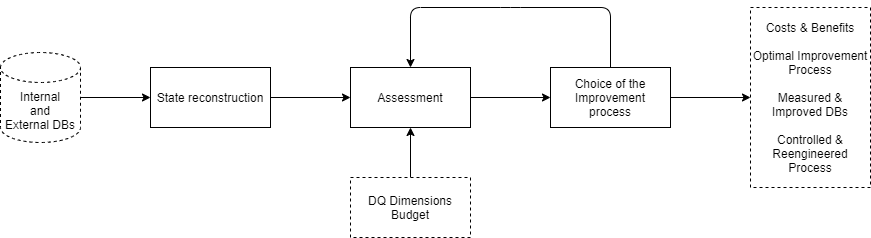
\includegraphics[width=0.9\textwidth]{figures/cdqm-diagram.png}
    \caption{Diagram of the CDQ methodology~\cite{batini2008}}
    \label{fig:cdqm-diagram}
\end{figure}
\FloatBarrier

\subsection{State reconstruction}

TODO

\subsection{Assessment}

TODO

\subsection{Choice of the optimal improvement process}

TODO

\section{BODQ}

Otto et al. (2011) developed a design process for the identification of business oriented DQ metrics~\cite{otto2011}.
The paper does not present any concrete DQ metrics even though they studied data quality problems in three companies.
Instead, those three companies' data problems were used to create an assumption that data defects cause business problems~\cite{otto2011}.
According to Otto et al. (2011), the identification of DQ metrics therefore should be based on how the data impacts process metrics~\cite{otto2011}.

A method engineering (ME) is used to design the framework.
Methodology therefore consists of five components:

\begin{itemize}
    \item design activities,
    \item design results,
    \item meta-model,
    \item roles and
    \item techniques.
\end{itemize}

\subsection{Meta-model}

Otto et al. (2011) describe entities and relations used to characterize the activities of the procedure model~\cite{otto2011}.

\begin{figure}[htb]
    \centering
    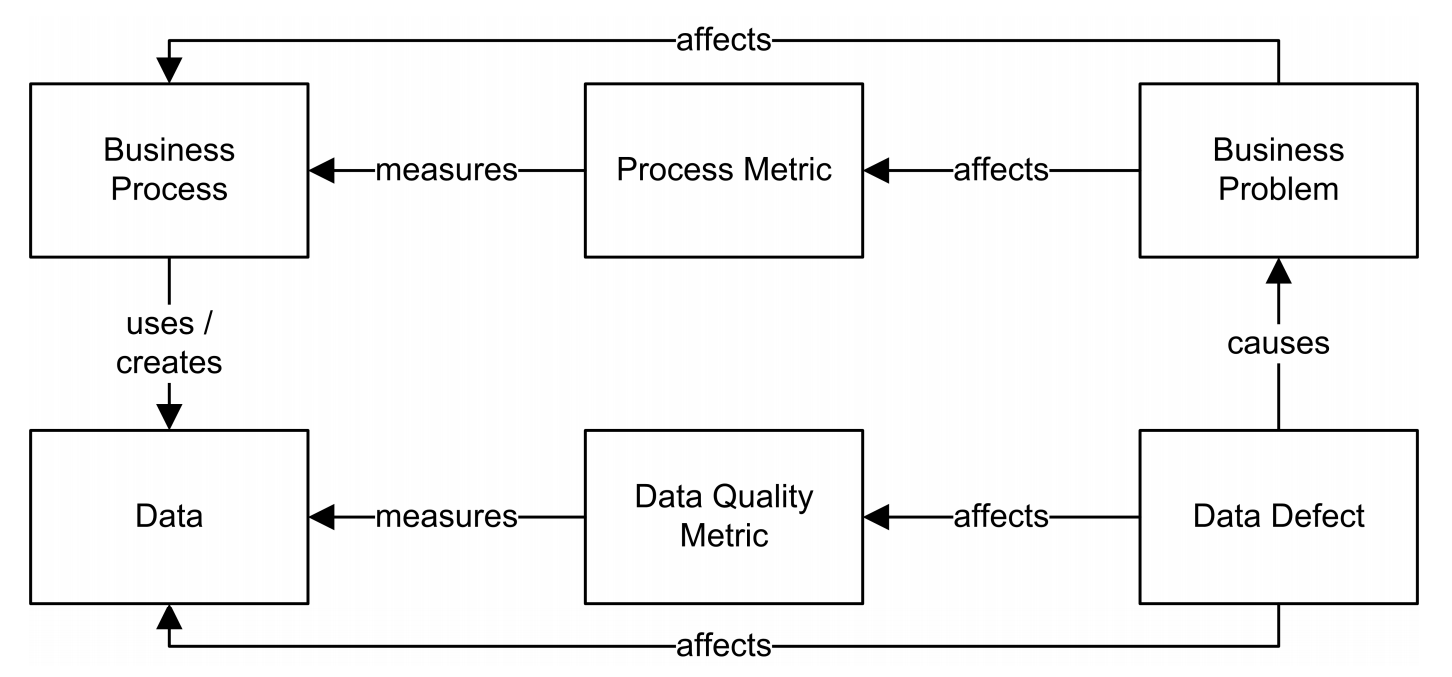
\includegraphics[width=0.9\textwidth]{figures/otto-figure-1.png}
    \caption{Entities and relations of a business oriented data quality metric~\cite{otto2011}}
    \label{fig:otto-figure-1}
\end{figure}
\FloatBarrier

\subsubsection{Business Problem}

Business problem is either system state (e.g. the package cannot be delivered) or incident (e.g. scrap parts production) causing decrease of system performance, therefore impacts \textit{process metrics} results.
It directly impacts business process and is defined by \textit{probability of occurence}\footnotemark and \textit{intensity of impact}\footnotemark.

\footnotetext[1]{Probability of occurence of event \( E \) can be denoted as \( P(E) = \frac{r}{n} \), where \( r \) is number of ways \( E \) can happen from all possible ways \( n \), \( P(E) \in [0, 1] \).}
\footnotetext[2]{
    Intensity of impact is a measure of the time-averaged power density of a wave at a particular location.
    In our case, intesity should be defined as \( I = \frac{\langle BC \rangle}{BA} \), where \( \langle BC \rangle \) is time-averaged business cost of problem and \( BA \) business area through which the problem propagates during certain time frame, \( I \in [0, \inf] \).
    If we define business area as sum of employees impacted by problem and their time spend to solve it, the unit of intensity would be costs per hour.
}

\subsubsection{Business Process}

By business process is meant sequence of tasks intended to generate value for customer and profit for the company.
The business process is controlled and defined as part of a~business strategy with corresponding modeling and measuring tools such as BPMN~2.0 or Key Performance Indicators (KPIs).

\subsubsection{Process Metric}

Quantitative measure of the degree to which a process fulfill a given quality attribute (e.g. scrap rate).

\subsubsection{Data}

Data is representation of objects and object relations.

\subsubsection{Data Defect}

It is an incident (e.g. wrong entered data), causing value decrease of data quality metrics.
As well as \textit{business problem}, a data defect poses a risk in terms of \textit{probability of occurence} and \textit{intensity of impact}.

\subsubsection{Data Quality Metric}

Quantitative measure of the degree to which data fulfill a given quality attribute (e.g. accuracy, consistency, currency,\ldots).

\subsection{Procedure Model}\label{subsec:procedure-model}

Procedure model defined by Otto et al. (2011) consists of three phases and seven activities.
Activity flow model is shown in the figure~\ref{fig:otto-figure-2}.
Letter color codes under the activities indicate degree of usage in the respective companies mentioned in the paper.
Black color means that activity was fully used, grey color means partial usage and white indicates no use at all.

\begin{figure}[htb]
    \centering
    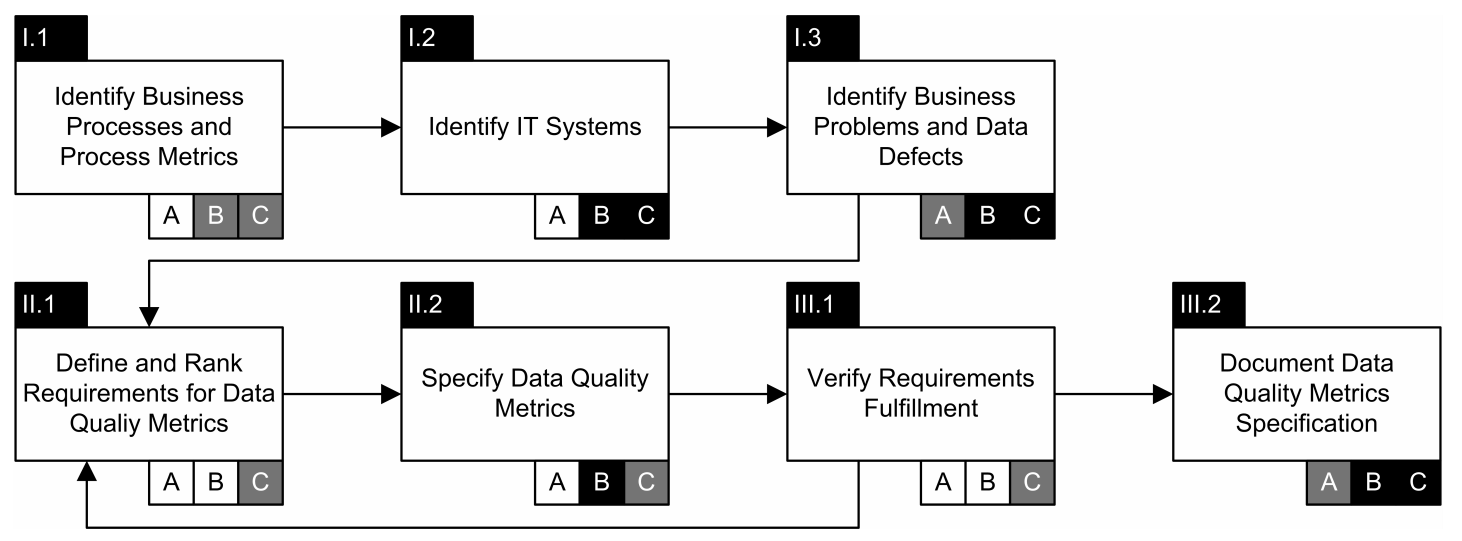
\includegraphics[width=0.9\textwidth]{figures/otto-figure-2.png}
    \caption{Procedure model and degree of usage of activities in each case~\cite{otto2011}}
    \label{fig:otto-figure-2}
\end{figure}
\FloatBarrier

\subsubsection{Phase 1}

First phase is used to collect information.
It consists of three activities:

\begin{enumerate}
    \item Identify Business Processes and Process Metrics,
    \item Identify IT Systems,
    \item Identify Business Problems and Data Defects.
\end{enumerate}

\subsubsection{Phase 2}

Second phase is used to specify requirements and design data quality mestrics.
It consists of two activities:

\begin{enumerate}
    \item Define and Rank Requirements for Data Quality Metrics,
    \item Specify Data Quality Metrics.
\end{enumerate}

\subsubsection{Phase 3}

Third phase is intended to approve and decument results.
As well assecond phase, this one consists of two activities:

\begin{enumerate}
    \item Verify Requirements Fulfillment,
    \item Document Data Quality Metrics Specification.
\end{enumerate}

\subsection{Roles}

In the last part, the authors declare six roles and their assignment to activities from section~\ref{subsec:procedure-model}.
Those roles are:

\begin{itemize}
    \item Chief Data Steward,
    \item Business Data Steward,
    \item Technical Data Steward,
    \item Process Owner,
    \item Process user and
    \item Sponsor.
\end{itemize}

\section{ORME}

Batini et al. (2007) provided DQ assessment methodology called ORME (from italian word \enquote{orme} meaning track or trace).
The methodology consists of four Data Quality Risk evaluation phases:

\begin{enumerate}
    \item prioritization,
    \item identification,
    \item measurement,
    \item monitoring.
\end{enumerate}

In the work, authors provided a comprehensive classification of costs of poor data quality.
In short, they categorized costs into three classes:

\begin{itemize}
    \item current cost of insufficient data quality,
    \item cost of IT/DQ initiative to improve current quality status,
    \item benefits gained from improvement initiative implementation.
\end{itemize}

\subsection{Prioritization}

In this phase the model reconstruction happen.
All the relationships among organization units, processes, services and data are put together and organized e.g. in the form of matrices (database/organization matrix, dataflow/organization matrix, database/process matrix).
The main goal is to provide map of the main data use across data providers, consumers and flows.

\subsection{Identification}

This phase main focus is on identification of loss events and definition of overall economic loss metrics.
In this case, loss can be expressed in 
\begin{enumerate*}[label=(\roman*)]
    \item absolute values (e.g. 100 USD),
    \item a percentage with respect to reference variables (e.g. 10\% of GDP), or
    \item a qualitative evaluation (e.g. low-medium-high).
\end{enumerate*}

\subsection{Measurement}

In this phase actual qualitative and quantitative assessment of data quality is conducted.

\subsection{Monitoring}

The last phase establishes a feedback loop and threshold in the DQ assessment process.
DQ dimensions should be, according to the authors, evaluated periodically.
Therefore quality rule violation allerts and automatic processes should be defined in order to ensure required DQ levels.

Authors suggest discriminant analysis as an easy and effective way of loss event identification.
The goal is to identify loss event based on set of new values in the data source.
The model is build on a training set, with two classes (\textit{loss} and \textit{no loss}) in consideration.
A set of linear functions from predictors is constructed,

\begin{equation*}
    L = b_1 x_1 + b_2 x_2 + \ldots + b_3 x_3 + c
\end{equation*}

where \( b_k \) are discriminant coeficient, \( x_k \) are input variables (predictors) and \( c \) is a constant.

\newpage
\section{Other}

\begin{figure}[htb]
    \centering
    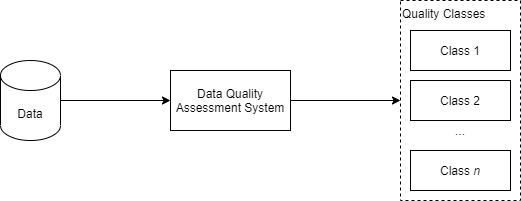
\includegraphics[width=0.9\textwidth]{figures/dq-simple.png}
    \caption{}
    \label{fig:dq-simple}
\end{figure}
\FloatBarrier

\begin{figure}[htb]
    \centering
    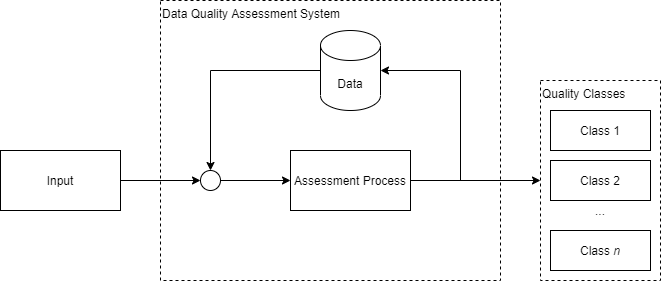
\includegraphics[width=0.9\textwidth]{figures/dq-system.png}
    \caption{}
    \label{fig:dq-system}
\end{figure}
\FloatBarrier

\section{Data Quality Attributes}

Eppler (2006) presented list of seventy of the most used data and information quality criteria explicitly defined in the literature.
They provide criterial basis for most of the DQ frameworks.
The list is shown in the figure~\ref{fig:dq-criteria}.

\begin{figure}[htb]
    \begin{multicols}{3}
        \begin{enumerate}
            \item Comprehensiveness
            \item Accuracy
            \item Clarity
            \item Applicability
            \item Conciseness
            \item Consistency
            \item Correctness
            \item Currency
            \item Convenience
            \item Timeliness
            \item Traceability
            \item Interactivity
            \item Accessibility
            \item Security
            \item Maintainability
            \item Speed
            \item Objectivity
            \item Attributability
            \item Value-added
            \item Reputation (source)
            \item Ease-of-use
            \item Precision
            \item Comprehensibility
            \item Trustworthiness\newline (source)
            \item Reliability
            \item Price 
            \item Verifiability
            \item Testability
            \item Provability
            \item Performance
            \item Ethics
            \item Privacy
            \item Helpfulness
            \item Neutrality
            \item Ease of Manipulation
            \item Validity
            \item Relevance
            \item Coherence
            \item Interpretability
            \item Completeness
            \item Learnability
            \item Exclusivity
            \item Right Amount
            \item Existence of meta information
            \item Appropriateness\newline of meta information
            \item Target group orientation
            \item Reduction of complexity
            \item Response time
            \item Believability
            \item Availability
            \item Consistent Representation
            \item Ability to represent null values
            \item Semantic Consistency
            \item Concise Representation
            \item Obtainability
            \item Stimulating
            \item Attribute granularity
            \item Flexibility
            \item Reflexivity
            \item Robustness
            \item Equivalence of redundant or distributed data
            \item Concurrency of redundant or distributed data
            \item Nonduplication
            \item Essentialness
            \item Rightness
            \item Usability
            \item Cost
            \item Ordering
            \item Browsing
            \item Error rate
        \end{enumerate}
    \end{multicols}

    \centering
    \caption{Data \& Information Quality Criteria~\cite{eppler2006}}
    \label{fig:dq-criteria}
\end{figure}
\FloatBarrier

Uniqueness
Accuracy
Consistency
Completeness
Timeliness
Currency
Format Compliance
Referential Integrity

Two main perspectives on Data Quality Management:

Broad Perspective (from the enterprise poin of view on the lifecycle of data circulating in the company)~\cite{book:dama}
Narrow Perspective (from the viewpoint of tasks to be done by data management professionals)~\cite{pres:dcam}

% \section{AI as a~tool for security breaches mitigation}\label{sec:ai-as-a-tool-for-security-breaches-mitigation}

%In the section~\ref{subsec:evasion} the principle of \textbf{model verifiability} was already mentioned.

\subsection{Parallel hybrid systems}\label{subsec:parallel-hybrid-systems}

In the paper \say{Is machine learning cybersecurity's silver bullet?} ESET's experts sort training data into three groups - malicious, clean and potentially unwanted.
They recommend not to use algorithm own output data as inputs, because any further errors are reinforced and multiplied, as the same incorrect result enters a~loop and creates more false positives or misses of malicious items.
In the next chapter ESET points out how crucial it is to achieve an equilibrium of sufficient protection from malicious items and false positives minimised to a~manageable level.
Finally, in the chapter \textit{Machine learning by ESET - The road to augur} authors let us take a~look under the hood of their ML engine called Augur.
For malicious file detection they are using two branches:
\begin{enumerate*}[label=(\roman*)]
    \item sandbox analysis followed by advanced memory analysis and behavioural features extraction (these features are later used to train ML models),
    \item ML-based branch.
\end{enumerate*}
ML-based branch consists of two methodologies:
\begin{enumerate*}[label=(\roman*)]
    \item neural networks, specifically deep learning and long short-term memory (LSTM),

    \item consolidated output of six classification algorithms.
\end{enumerate*}
While consolidating output of those six classification algorithms, two modes (setups) are used.
The first one is used for security critical environments, making algorithm more likely to mark file as malicious if most of the previous algorithms vote it as such.
The other setup is more conservative - labelling a~sample clean if at least one algorithm comes to such conclusion.

\subsection{Serial hybrid systems}\label{subsec:serial-hybrid-systems}

\begin{enumerate}[label=(\roman*)]
    \item exposure prevention (network filtering),
    \item pre-execution detection based on machine learning,
    \item runtime control proactively looking out for suspicious behavior of devices in the network (behavioral analysis based on ML),
    \item automated response such as \textit{automatic rollback} to help restore systems to their pre-attack state, system disinfection techniques or Incident of Compromise (IoC) scanning~\cite{whitepaper:kaspersky_next_generation}.
\end{enumerate}

Features are extracted from items in hard regions, to undergo ML classifiaction.
Various types of models are pre-trained with human annotated data.
Which model is selected for classification of items in region depends on several factors - extractable features, type of objects, etc.

Second topic relate to data integrity.
There is serious concern that attackers can inject data while a~model is in the training stage to alter the inference capability or add disturbance into the input samples to change model's interpretation and distort result.

Other option is to append additional component to capture and therefore filter out malicious input sample before it gets into inference stage - \textbf{adversarial sample detection}.
Simple deterministic detector could be a~deterministic comparer having some type of \textit{distance} as a~criterion.
Detectors vary greatly - forming a~group of independent models worth exploring in other papers.
% possibility to write more about detectors - the detection model may extract related information at each layer of the original model to perform detection based on the extracted information

A deformed input samples does not effect normal classification function of a~model.
\textbf{Input reconstruction} works by deforming input samples to defend against evansion attack by adding noise, de-noising, or using an automatic encoder (a type of artificial neural network)~\cite{huawei_security}.

Last but not least method is \textbf{model verification}.
In general, verification is a~discipline of software engineering with goal to assure that software fully satisfies all the expected requirements.

\textbf{Regression analysis} methods such as linear and ordinary least squares regression are ideal to detect noise and abnormalities in the data sets.
Thanks to relative directness presents those methods easy way to fight back data poisoning attack.

\textbf{Ensemble analysis} points out that usage of multiple sub-models - each one of them trained with different training data set - reduces probability of system being affected by poisoning attacks greatly.

\begin{enumerate}
    \item \textbf{Explainable data}
    As Huawei in its paper mentions, if several representative characteristics can be found at data sets and those features are carefully selected, then a~some models can be meaningfully interpretted~\cite{huawei_security}.
    Of course, data set are not usually simple enough to make such analysis.
    Moreover, AI model can grow in complexity and even with understandable data and features in the beggining, there is no guarantee that result is intereprettable in the end.

    \item \textbf{Explainable model}
    Some of the ML models (either for classification or regression) are interprettable naturaly.
    Their typical properties are \textit{linearity}, \textit{monotonicity} and \textit{interaction features} - possibility to manually add non-linearity into the model.
\end{enumerate}

\subsection{Data security}\label{subsec:data-security}

In addition to model and architecture security mechanism, we have to consider security of data sets.
Data often contains personal information of users - so called \textit{sensitive attributes}.
Such information can be in a~form of personal identifiers or quasi-identifiers.
\textit{Personal identifier} is an unique information that identifies a~user - a~birth number, bank account number and other types of personal IDs.
\textit{Quasi-identifiers} are characteristics which needs to be used in combination with others to identify an entity - examples are gender, postal code, age or nationality.

To prevent data stealing and following re-identification of users, several models exists to protect personal information of individuals in dataset.
Those privacy models are \textbf{optimal k-anonymity}, \textbf{l-diversity}, \textbf{t-closeness} and \textbf{differential privacy}.
Three general types of attack to datasets exists:
\begin{enumerate*}[label=(\roman*)]
    \item \label{itm:reident} re-identifying an individual,
    \item \label{itm:query} query whether an individual is a~member of a~dataset,
    \item \label{itm:linking} linking an individual to a~sensitive attribute.
\end{enumerate*}

\textbf{Optimal k-anonymity} protects against both cases~\ref{itm:reident} and~\ref{itm:query} by transforming quasi-identifiers so that at least \( k - 1 \) members of set are indistinguishable from each other - group based anonymization.
Identifiers are transformed by suppression (needless attributes are replaced with \textit{dummy} values) and generalization (individual values of attributes are replaced with a~broader category - e.g.\ specific age can be replaced by a~range).
As \( k \) increases risk of data exploit reduces, on the other hand data quality decreases - we are talking about a~\textit{privacy-utility} tradeoff.
Moreover, the \( k \) is limit - in order for this method to work if \( k \) is set to \( k \triangleq 10 \) then any group must contain at least \( 10 \) individuals.
The first drawback of k-anonymity is vulnerability to \textit{homogeneity attack} which works on premise of data having sensitive value identical within a~set of \( k \) records - it is enough to find the group of records, the individual belongs to, if all of them have the same sensitive value.
Second drawback is the possibility of \textit{background knowledge attack} where attacker identifies associations among one or more quasi-identifiers and reduces the set of possible values for the sensitive attribute.

Both \textbf{l-diversity} and \textbf{t-closeness} are group based anonymization techniques building on a~concept of \textbf{optimal k-anonymity}.
In addition to \textbf{optimal k-anonymity}, \textbf{T-closeness} transforms quasi-identifiers such that each group is within a~distance \( t \) of the distribution of sensitive values for the entire dataset~\cite{web:privacy-models}.
The distance is measured as the cumulative absolute difference of the distributions, as \( t \) decreases both risk of sensitive attribute disclosure and data quality decreases.
Suppose that the sensitive attribute is salary.
Each group's frequency distribution of salary will be within a~distance \( t \) from the salary frequency distribution for the entire dataset~\cite{web:privacy-models}.

\textbf{Differential privacy} and its variants (epsilon, epsilon-delta) are statistical techniques aiming to protect data against \textit{differentiated attack}.
The model guarantees that even if someone has complete information about 99 of 100 people in a~data set, they still cannot deduce the sensitive information about the final person~\cite{web:differential-privacy}.
The mechanism works by adding random noise to the aggregate data, leaving only a~trend without possibility to figure out exact values in data (e.g.\ information that \( n\% \) of users prefer some product over another).

\subsection{Data Quality Rules}

There are a number of general data quality rules one can deduce from a Feedback-Control Systems view of information systems~\cite{orr1998}.

\begin{enumerate}
    \item Unused data cannot remain correct for very long;
    \item data quality in an information system is a function of its use, not its collection;
    \item data quality will, ultimately, be no better than its most stringent use;
    \item data quality problems tend to become worse as the system ages;
    \item the less likely some data attribute (element) is to change, the more traumatic it will be when if finally does change;
    \item laws of data quality apply qually to data and metadata.
\end{enumerate}

\subsection{System Stability}

In principle, we can classify three types of system stability:

\begin{enumerate}
    \item Stable System (Absolute and Conditional stability);
    \item Marginally Stable System;
    \item Unstable System.
\end{enumerate}

\subsection{Analytics Types}

\begin{itemize}
    \item Descriptive – what happened in the past;
    \item Diagnostic – why something happened in the past;
    \item Predictive – what is most likely to happen in the future;
    \item Prescriptive – recommends actions to affect those outcomes.
\end{itemize}

\subsection{Differential Privacy}

DQ dimensions vs DQ metrics

"Confidetial/secret data will always have limited quality."
